% (c) 2014 Daniele Zambelli - daniele.zambelli@gmail.com

\chapter{Foglio di calcolo}

\section{Avviamo ``Calc''}

\emph{Perché un foglio di calcolo}

In molti ambiti gli umani sono costretti ad effettuare molti calcoli,
pensiamo solo all'economia, alla ricerca scientifica o statistica,
alla progettazione, ...
I matematici spesso hanno realizzato strumenti per semplificare i calcoli,
inventando i computer hanno trovato il modo di far fare \emph{completamente} i
calcoli a qualcun altro: al computer.

Se dobbiamo eseguire molte operazioni è più sicuro (e meno noioso),
farle fare ad un elaboratore elettronico. Ma come convincere un
calcolatore a fare i calcoli per noi? Il modo più semplice è quello di
avviare un apposito programma che si chiama genericamente
``foglio di calcolo''.

Ne esistono molti in commercio, noi ci riferiremo a ``Calc'' che è il
foglio di calcolo del programma di ufficio: ``Libre Office'' (o ``Open Office'').
Se non avete ``Libre Office'' nel vostro computer, fatevi aiutare da qualcuno
esperto e installatelo, è facile.
Il programma si scarica gratuitamente da Internet ed è un \emph{software libero}.

\begin{inaccessibleblock}[Figura: TODO]
 \begin{figure}[htbp]
\centering
%  \includegraphics[scale=0.6]{/informatica/05_01_f_di_calc/00_calc.png}
% \end{inaccessibleblock}
% \begin{inaccessibleblock}[Figura: TODO]
% \begin{inaccessibleblock}[Figura: TODO]
%  \includegraphics[scale=0.6]{chap/05informatica/01_fogliodicalcolo/img/00_calc.png}
% \end{inaccessibleblock}
\begin{inaccessibleblock}[Figura: TODO]
 \includegraphics[scale=0.6]{img/00_calc.png}
\end{inaccessibleblock}
\caption{Come si presenta una finestra di Calc.}
\end{figure}
\end{inaccessibleblock}

Una volta trovato (o installato) \emph{Libre Office} avviate il programma ``Calc''.
Vi troverete davanti un foglio di calcolo e tutta una cornice che contiene
gli strumenti per gestirlo, dall'alto in basso possiamo riconoscere:

\begin{itemize} [noitemsep]
\item il menu;
\item {}
la barra delle icone (individuate l'icona per salvare il lavoro,
per stampare il foglio, per le operazioni di taglia-copia-incolla, ...);
\item la barra di formattazione;
\item la barra di immissione;
\item i bordi del foglio;
\item il foglio vero e proprio;
\item la barra di stato.
\end{itemize}

Nei seguenti paragrafi vedremo cosa è e come si usa un \emph{foglio di calcolo}.

\section{Celle, colonne, righe... il foglio di calcolo}
\label{05_01_f_di_calc:celle-colonne-righe-il-foglio-di-calcolo}

\emph{Cos'è, e come usare le funzioni di base di un foglio di calcolo.}

Un Foglio di Calcolo è un'immensa tabella composta da alcune migliaia di
righe e alcune centinaia di colonne che generano una grande quantità di
celle nei loro incroci.
L'elemento base di un Foglio di Calcolo, è dunque la cella.
Ogni cella ha: un indirizzo, un contenuto e un  formato:

\paragraph{Indirizzo}

Come nella battaglia navale l'indirizzo di ogni cella è composto da una
lettera seguita da un numero, ad es. B3 è la cella che si trova all'incrocio
della seconda colonna con la terza riga. Poiché le lettere sono solo 26 e
noi, a volte, abbiamo bisogno di più colonne, arrivati alla lettera ``Z''
proseguiamo con ``AA'', ``AB''... e così via.
Nella \emph{barra di immissione}, in alto a sinistra viene visualizzato
l'indirizzo della cella in cui ci troviamo.
Cliccando in diverse celle si può osservare l'indirizzo che cambia.

\paragraph{Contenuto}

Ogni cella può avere un contenuto che è uno di questi 3 oggetti:

\begin{itemize} [noitemsep]
\item Parole, una stringa qualunque.
\item Numeri che possono rappresentare anche percentuali, ore o date.
\item {}
Formule, espressioni che iniziano con un uguale. Quando si termina di
inserire una formula, nella cella viene mostrato il risultato del calcolo,
mentre il testo della formula appare nella parte alta dello schermo nella
barra di immissione.
\end{itemize}

Gli operandi delle formule, possono essere numeri o indirizzi di celle.
Quando viene modificato il contenuto di una cella, tutte
le formule che contengono il suo indirizzo vengono ricalcolate.

\paragraph{Formato}

Ogni cella ha diversi attributi che riguardano il suo formato o quello del
suo contenuto.
Ci sono decine di aspetti che possono essere modificati con
il formato della cella:

\begin{itemize} [noitemsep]
\item colore di sfondo;
\item bordo;
\item dimensioni;
\item font, colore, dimensione dei caratteri;
\item formato dei numeri;
\item allineamento del contenuto;
\item ...
\end{itemize}

Possiamo applicare queste prime informazioni per realizzare un formulario di
geometria che calcoli perimetri e aree di vari poligoni.
Apriamo un nuovo foglio di calcolo. Prima ancora di incominciare a riempirlo
lo salviamo con nome:

\emph{Menu-File-Salva Come}.

Conviene salvarle il documento
in una nostra cartella e darle per nome ``quadrilateri''.
Per salvare un file basta anche cliccare sull'icona con un dischetto,
di solito terza da sinistra o più rapidamente ancora premere il tasto:

\emph{\textless{}Ctrl-s\textgreater{}}.

L'obiettivo è avere un foglio nel quale inserire alcuni dati relativi ai
quadrilateri notevoli e calcolare altre informazioni relative alla figura.
Possiamo distinguere con un colore di sfondo le celle nelle quali inserire
dati e con un altro colore quelle che conterranno i risultati.
Dovremo adattare la larghezza delle colonne a seconda dello spazio occupato
dal contenuto.
Potrebbe anche essere utile graficamente separare i vari problemi
riquadrando con un bordo le relative celle.
Di seguito riporto dei suggerimenti per l'inizio del lavoro:

\begin{itemize} [noitemsep]
\item \texttt{A1: Formulario di geometria: i quadrilateri}
(dimensione e colore a fantasia)
\item \texttt{A3: Problemi sul Quadrato} 
(grassetto, colorato)
\item \texttt{A5: Dato il lato, trovo: perimetro, area e diagonale}
(grassetto, corsivo)
\item \texttt{A6: Lato:}
(allineamento a destra)
\item \texttt{B6: }
(colore di sfondo: verde)
\item \texttt{A7: Perimetro}
(allineamento a destra)
\item \texttt{B7: =B6 * 4}
(colore di sfondo: azzurro)
\item \texttt{A8: Area}
\item \texttt{B8: =B6\textasciicircum{}2}
(colore di sfondo: azzurro)
\item \texttt{A9: Diagonale}
\item \texttt{B9: =B6*sqrt(2)}
(colore di sfondo: azzurro)
\item \texttt{A1:B9}
(Menu-Formato-Cella-Bordo: contorno)
\end{itemize}

\emph{Questo è un buon momento per salvare il lavoro fatto.}

Prima di procedere con il formulario conviene provare inserendo nella cella
\texttt{B6} diversi valori numerici prima semplici per controllare che il foglio
esegua calcoli corretti, poi più strani, con la virgola, molto grandi o
molto piccoli e osservare i corrispondenti risultati.
Una volta risolti eventuali problemi riscontrati, possiamo salvare il lavoro
fatto e passare ai problemi inversi del quadrato oppure
affrontare i problemi relativi ad altre figure geometriche.

\textbf{Riassumendo}

\begin{itemize} [nosep]
\item 
Un foglio di calcolo è composto da un gran numero di ``celle'' organizzate
in ``righe'' e ``colonne''
\item 
Ogni cella è caratterizzata da:
\begin{itemize} [nosep]
\item 
un indirizzo, composto da una lettera o gruppo di lettere e un numero;
\item 
un contenuto, che può essere:
\begin{itemize}
\item 
un testo,
\item 
un numero,
\item 
una formula;
\end{itemize}
\item 
un formato.
\end{itemize}
\end{itemize}

\section{Formati e ordinamenti}
\label{05_01_f_di_calc:formati-e-ordinamenti}

\emph{Come selezionare un blocco di celle, sommare i dati di un intero blocco,
modificare la larghezza di una colonna, disegnare griglie,
ordinare i dati.}

Spesso nei fogli di calcolo si devono inserire formule con molti operandi o
molte formule che si assomigliano, i fogli di calcolo forniscono degli
strumenti per realizzare ciò in modo efficiente e veloce.
Come primo esempio partiamo dai dati relativi alla superficie dei continenti
e alla loro popolazione. Per ora lavoreremo su pochi dati, ma cerchiamo di
ragionare pensando di avere a che fare con centinaia di righe di dati
invece che con solo queste sei.

\begin{inaccessibleblock}[Figura: TODO]
 \begin{figure}[htbp]
\centering
\begin{inaccessibleblock}[Figura: TODO]
 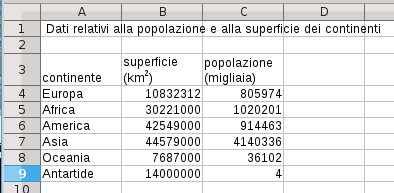
\includegraphics[scale=0.8]{img/01_calc.png}
\end{inaccessibleblock}
\caption{Dati relativi alla superficie e alla popolazione dei 6 continenti.}
\end{figure}
\end{inaccessibleblock}

Avviamo un nuovo foglio e salviamolo con il nome ``continenti''.
Poi eseguiamo le seguenti istruzioni:

\begin{itemize} [noitemsep]
\item \texttt{A1: Dati relativi alla popolazione e alla superficie dei 
continenti}
(dimensione e colore a fantasia)
\item \texttt{A3:C10}:
Ricopiamo i dati della tabella riportata sopra.
\end{itemize}

Non è difficile ricopiare la tabella, si incontra qualche
difficoltà solo nelle celle \texttt{B3} e \texttt{C3}.

\begin{itemize} [noitemsep]
\item 
La cella \texttt{B3} contiene un carattere posto a indice, come ottenerlo?
Innanzitutto si scrivono tutti i caratteri che vogliamo appaiano:
``Area (km2)'', poi con il mouse selezioniamo nella riga di immissione
il solo carattere ``2'' e da \texttt{Menu-Formato-Carattere-Posizione} scegliamo
``apice''. Confermando con invio otteniamo il risultato desiderato.
\item 
La cella \texttt{C3} contiene una scritta troppo lunga che esce dai bordi della
cella stessa, vorremmo che fosse spezzata su due righe. Poniamoci in \texttt{C3}
e modifichiamo il formato della cella:
\texttt{Menu-Formato-Celle-Allineamento-Scorrimento testo automatico}.
\end{itemize}

\emph{Questo è un buon momento per salvare il lavoro fatto.}

Ora vogliamo che il contenuto di queste celle sia visualizzato in grassetto
e sia centrato: dopo aver selezionato le celle, tra le icone che si trovano
nella \emph{barra di formattazione} troviamo i pulsanti giusti da cliccare per
ottenere questi effetti.
Possiamo ripetere queste operazioni per ognuna delle celle oppure...
{[}Gli informatici sono estremamente pigri (addirittura più dei matematici),
poiché odiano ripetere le stesse operazioni e gli stessi gesti hanno
inventato delle macchine bravissime a ripetere stupide operazioni.{]}
Invece che modificare per tre volte il formato di una cella è possibile
selezionare le tre celle e aggiustarne il formato assieme.

Per selezionare un gruppo di celle contiguo e rettangolare basta cliccare
sulla cella in alto a sinistra e, tenendo premuto il tasto sinistro del
mouse, trascinare il cursore fino alla cella in basso a destra.
Quando si rilascia il tasto del mouse il colore delle celle selezionate
apparirà invertito.

Ora vogliamo aggiungere una riga che contenga i totali della superficie e
della popolazione:

\begin{itemize} [noitemsep]
\item \texttt{B11: =somma(B4:B9)} (grassetto)
\item \texttt{C11: =somma(C4:C9)} (grassetto)
\end{itemize}

Se ora effettuiamo un doppio clic nella cella \texttt{B10} ci viene evidenziata 
la
formula e la zona di celle su cui lavora.

Dato che la somma di un gruppo contiguo di celle è molto frequente, ci sono
molti modi per immettere queste formule. Proviamo a vederli, poi, a seconda
dei casi useremo quello più comodo. 
Per prima cosa cancelliamo il contenuto delle celle \texttt{B10:C10}.
Ci riportiamo nella cella \texttt{B10} e: iniziamo a scrivere la formula:

\texttt{=somma(}

selezioniamo con il mouse le celle \texttt{B4:B10},
chiudiamo la parentesi tonda e confermiamo con il tasto 
\texttt{\textless{}Invio\textgreater{}}

Per la cella \texttt{C11} proviamo ad usare un altro metodo.
Una volta portati nella cella \texttt{C11}, clicchiamo l'icona della 
\emph{sommatoria}
che si trova in alto a sinistra della casella di inserimento se le scelte
di Calc ci vanno bene, confermiamo la formula con il tasto 
\texttt{\textless{}Invio\textgreater{}}.

\emph{Questo è un buon momento per salvare il lavoro fatto.}

I numeri con troppe cifre sono difficili da leggere e valutare,
per facilitare questo compito, di solito, si separano le cifre a gruppi di 3
con dei puntini, i separatori delle migliaia
(delle virgole per gli anglosassoni che
usano invece il punto per separare la parte intera da quella decimale).
Selezioniamo le celle da \texttt{B4} a \texttt{C10} e da 
\texttt{Menu-Formato-Celle-Numeri}
scegliamo il numero con il separatore delle migliaia e senza cifre decimali.

I caratteri con cui stiamo lavorando sono piuttosto piccoli, vogliamo
aumentare la dimensione della font dei caratteri per tutte le celle del
foglio. Per selezionarle tutte in un solo colpo possiamo cliccare
nell'angolo della cornice con le intestazioni delle righe e delle colonne,
il rettangolino che si trova sopra a ``1'' e a sinistra di ``A''. Una volta
selezionato tutto il foglio di lavoro, nella barra di formattazione cambiamo
la dimensione del font da 10 a 12.

A questo punto può succedere un effetto spiacevole: alcune celle
dove prima c'era un numerone ora appaiono tre \emph{cancelletti}: ``\#\#\#''.
Cosa è successo? Se una cella non è abbastanza grande per contenere un
numero questo non viene tagliato.
Poiché non è accettabile che un numero venga visualizzato solo in parte,
quando non può essere contenuto in una cella, viene sostituito da un simbolo
convenzionale: ``\#\#\#''.
Per vedere di nuovo il nostro numero possiamo seguire una delle seguenti
strade:

\begin{enumerate} [noitemsep]
\item togliere i puntini delle migliaia;
\item diminuire le dimensioni del carattere;
\item allargare la cella.
\end{enumerate}

La soluzione più adatta nel nostro caso è la terza.
Clicchiamo con il tasto destro del mouse sull'intestazione della colonna da
allargare e dal menu a tendina che appare scegliamo la voce:
``Larghezza colonna''.
Nel campo di inserimento al posto di 2,62 scriviamo 3 e confermiamo.
La colonna si sarà allargata un pochino e i numeri verranno di nuovo
visualizzati.

\emph{Questo è un buon momento per salvare il lavoro fatto.}

A volte può essere utile avere i dati ordinati rispetto ad un certo criterio.
Se i continenti fossero decine o centinaia, per trovare i dati relativi ad
uno di questi sarebbe comodo averli scritti in ordine alfabetico.
Possiamo dire \emph{Calc} di ordinare le righe in base
al contenuto di una colonna.
Se vogliamo ottenere i continenti in ordine alfabetico selezioniamo il blocco
di celle da \texttt{A4:C9} e attraverso il \texttt{Menu-Dati-Ordina} scegliamo 
come
primo criterio la colonna ``A''.
Confermando, otteniamo le righe ordinate in ordine alfabetico dall'Africa
all'Oceania.

Se vogliamo i continenti ordinati dal più popolato al meno popolato, sempre
dopo aver selezionato tutte le celle che contengono i dati da ordinare,
scegliamo dal \texttt{Menu-Dati-Ordina} come primo criterio la colonna 
\texttt{C} e
come ordine quello discendente.
In un batter d'occhio ritroveremo i nostri dati ordinati per popolazione.

\textbf{Riassumendo}

\begin{itemize} [nosep]
\item È possibile selezionare un blocco di celle con il mouse o con la tastiera.
\item È possibile assegnare un formato a tutte le celle di un blocco.
\item È possibile calcolare la soma dei numeri contenuti in blocchi di celle.
\item È possibile disegnare i contorni delle celle.
\item Si può ordinare un blocco di celle in base a diversi criteri.
\item Spesso ci sono molti modi diversi per eseguire la stessa operazione.
È importante saper usarne uno, poi gli altri si imparano con il tempo e
con l'uso.
\end{itemize}

\section{Copiare in modo intelligente}
\label{05_01_f_di_calc:copiare-in-modo-intelligente}

\emph{Come ricopiare formule usando indirizzi relativi e assoluti.}

Riprendiamo i dati già usati nel capitolo precedente, con delle semplici
formule possiamo ottenere delle informazioni nuove.
Possiamo, ad esempio, far calcolare la densità di popolazione per mezzo
della formula popolazione/superficie.

\begin{itemize} [noitemsep]
\item \texttt{D3: Densità ab/km2} 
(centrato, grassetto)
\item \texttt{D3:} Selezionare nella riga di input il solo~2 
(formato-carattere-posizione-apice)
\item \texttt{D3:} 
(formato cella-allineamento-acapo automatico)
\item \texttt{D4: =C4*1000000/B4}
(formato-celle-numeri- zero decimali)
\item \texttt{D5: =C5*1000000/B5}
(formato-celle-numeri-zero decimali)
\item \texttt{D6:} \dots
(\dots)
\end{itemize}

Dato che i continenti sono solo 6 non è un grande problema scrivere le 6
formule diverse una sotto l'altra, ma in un foglio di calcolo spesso si 
devono scrivere centinaia o migliaia di formule simili a queste!
Chi ha progettato il foglio di calcolo ha previsto degli strumenti che
permettono di ricopiare velocemente le formule.
Ponendoci nella cella \texttt{D4},
appare nell'angolo in basso a destra, della cella stessa, un quadratino nero;
con il mouse trasciniamo questo quadratino verso il basso fino a coprire
tutte le celle in cui vogliamo ricopiare la formula.

Non solo il programma ha ricopiato la formula ma ha anche aggiustato gli
indici, proprio come ci serviva.
Da notare che quando viene ricopiata una formula vengono anche ricopiati i
formati della celle in cui la formula è stata scritta.

\emph{Questo è un buon momento per salvare il lavoro fatto.}

Un'altra informazione interessante che possiamo ricavare dai pochi dati in
nostro possesso è la percentuale rappresentata dalla superficie di un
continente rispetto alla superficie totale delle terre emerse.
La percentuale non è altro che un rapporto, il quoziente tra la superficie
di un continente e il totale.
Procediamo con il lavoro:

\begin{itemize} [noitemsep]
\item \texttt{E3: Perc. Sup.} (centrato, grassetto)
\item \texttt{E4: =B4/B10}
\end{itemize}

Il risultato di questo calcolo è un numero compreso tra zero e uno,
non è certo la percentuale cercata,
se lavoriamo sulla carta, per trasformare questo numero nella percentuale
basta moltiplicarlo per \texttt{100}. Nei fogli di calcolo basta indicare nel
formato della cella che quel numero deve essere inteso come una percentuale:

\begin{itemize} [noitemsep]
\item \texttt{E4: =B4/B10}
(formato-celle-numeri-percentuale)
\item \texttt{E5: =B5/B10}
(formato-celle-numeri-percentuale)
\item \dots
\end{itemize}

Anche qui, invece di riscrivere tutte le formule possiamo sfruttare le
capacità del foglio di calcolo e farle ricopiare verso il basso.
Dopo esserci posizionati nella cella \texttt{E4}, prendiamo il quadratino che
appare in basso a destra e trasciniamolo verso il basso in modo da coprire
le celle di tutti i continenti.
Questa volta l'effetto non è quello desiderato:
otteniamo una serie di errori! Come mai?

Osserviamo una delle celle in cui è comparso l'errore, la cella
\texttt{E5} contiene la formula \texttt{=B5/B12}.
Per capire meglio la formula selezioniamo la cella con un doppio clic.
Vengono evidenziate in rosso e blu le celle che sono utilizzate nella formula
stessa.
Appare evidente che \texttt{B5} va bene, ma \texttt{B11} doveva essere 
\texttt{B10}!
Nella cella \texttt{B12} non c'è niente e il foglio di calcolo la interpreta
come se contenesse il valore \texttt{0}.
Giustamente produce un errore di divisione per \texttt{0}.

Noi vogliamo che, nel ricopiare le formule, l'indice numerico di \texttt{B4} 
venga
modificato ma quello di \texttt{B10} rimanga costante.
Nei termini dei fogli di calcolo si dice che \texttt{B4} deve essere un
\textbf{indirizzo relativo}, \texttt{B10} un \textbf{indirizzo assoluto}.
Per essere pignoli a noi non occorre che tutto \texttt{B10} sia assoluto,
siccome vogliamo ricopiare la formula verso il basso ci basta che sia
assoluta la parte numerica dell'indirizzo: l'\texttt{10}.

Per comunicare questi desideri al foglio di calcolo si mette davanti
al riferimento che vogliamo sia assoluto il carattere dollaro: ``\$''.
Questo fa si che il programma quando ricopia le formule non ne modifichi
il riferimento.
Aggiustiamo le nostre formule:

\begin{itemize} [noitemsep]
\item \texttt{E4: =B4/B\$11}
(formato-celle-numeri-percentuale)
\end{itemize}

Ora ricopiare la cella verso il basso produce l'effetto desiderato!
Nella cella \texttt{E5} ci sarà la formula \texttt{=B5/B\$10},
nella cella \texttt{E6} la formula \texttt{=B6/B\$10}, e così via.

L'elaborazione numerica dei nostri dati è completa,
disegniamo un bordo anche attorno alle nuove celle che abbiamo
riempito ottenendo così un foglio presentabile.

\emph{E salviamo il lavoro fatto.}

\textbf{Riassumendo}
\begin{itemize} [nosep]
\item 
Si possono ``ricopiare'' formule trascinando il quadratino che appare in
basso a destra di una cella selezionata.
\item 
Quando ricopiamo una formula verticalmente gli indici relativi alla riga,
i numeri, vengono modificati.
\item 
Quando ricopiamo una formula orizzontalmente gli indici relativi alla
colonna, le lettere, vengono modificati.
\item 
Se vogliamo che, nel ricopiare una formula, un indice non venga modificato,
basta che lo facciamo precedere dal carattere: ``\$''.
\end{itemize}

\section{Diagrammi}
\label{05_01_f_di_calc:diagrammi}

\emph{Come rappresentare graficamente i dati.}

Spesso un grafico dà una più immediata comprensione di un fenomeno rispetto
ad una lista di numeri.
I fogli di calcolo permettono di disegnare grafici di diversa forma.

Riprendendo il foglio dei continenti vogliamo aggiungere due grafici per
rappresentare la superficie e la popolazione.

Apriamo il foglio su cui abbiamo lavorato finora selezioniamo le celle che
contengono i dati che vogliamo rappresentare.
Iniziamo costruendo un grafico a torta che riporti la superficie dei
diversi continenti.

\begin{enumerate} [noitemsep]
\item Selezioniamo le celle \texttt{A4:B9}.
\item Da menu scegliamo Inserisci-Diagramma, viene così aperta una finestra
di dialogo che ci guida nella definizione del diagramma.
\item Controlliamo che sia selezionata la casella
``Prima colonna come didascalia'' e premiamo ``Avanti''.
\item Nella seconda pagina di questo dialogo selezioniamo:
``Rappresenta oggetti nell'anteprima'',
e scegliamo il grafico a torta e ``Serie di dati in Colonne''.
\item Nella terza pagina, scegliamo ``normale''.
\item Nell'ultima pagina scriviamo il titolo (ad es. ``Superficie'')
e confermiamo cliccando sul bottone ``Crea''.
\end{enumerate}

A questo punto viene creato un diagramma. Un clic sul diagramma lo seleziona
e fa apparire le maniglie di dimensionamento che permettono di modificarne
le dimensioni.
Quando è selezionato possiamo anche spostarlo dove vogliamo che appaia nella
nostra pagina. Posizioniamolo subito sotto ai dati.

\emph{Questo è un buon momento per salvare il lavoro fatto.}

È possibile modificare i dati rappresentati nel diagramma cliccando con il
tasto sinistro sul diagramma stesso e scegliendo, dal menu contestuale,
la voce ``Modifica area dati''.

Se vogliamo che il diagramma sia riquadrato da un bordo, dopo aver dato un
doppio clic sul diagramma, scegliamo dal menu contestuale la voce ``Area del
diagramma''.

Se vogliamo modificare più profondamente il diagramma appena creato possiamo
effettuare un doppio clic sul diagramma stesso.
Il menu principale del foglio di calcolo cambia e cambiano anche i menu
contestuali (quelli legati al tasto destro) a seconda di cosa viene puntato
dal mouse.
Dal menu ``Inserisci'' scegliamo ``Legenda'' e togliamo il segno di spunta su
``Visualizza''.

La Legenda scompare, ma adesso il diagramma è di difficile interpretazione,
operiamo dunque un'altra modifica:
sempre dal menu Inserisci scegliamo ``Etichette'' e chiediamo che ci vengano
mostrati i valori come percentuale e anche le etichette di testo.
Se le etichette sono troppo lunghe e sbilanciano la rappresentazione conviene
abbreviarle.
Ora se il diagramma risulta troppo piccolo e non riempie bene lo spazio
a sua disposizione possiamo cliccare vicino alla \emph{torta} e allargarlo
agendo sulle maniglie verdi che appaiono.

\emph{Questo è un buon momento per salvare il lavoro fatto.}

Ora se vogliamo un diagramma che contenga i dati relativi al numero di
abitanti dobbiamo selezionare i nomi dei continenti e i valori della
popolazione.
Purtroppo questi valori non sono contigui, per selezionarli
dobbiamo usare un trucco:

\begin{enumerate} [nosep]
\item selezioniamo con il mouse le celle \texttt{A4:A9} e
\item selezioniamo le celle \texttt{C4:C9} tenendo premuto contemporaneamente
il tasto \texttt{\textless{}Ctrl\textgreater{}}.
\end{enumerate}

Il tasto \texttt{\textless{}Ctrl\textgreater{}} permette di effettuare selezioni 
multiple su blocchi
rettangolari non contigui.
Dopo aver selezionato le aree contenenti i dati,
dal \texttt{menu-Inserisci} scegliamo la voce ``Diagramma''.
Questa volta invece che un diagramma a torta vogliamo un istogramma.
Come prima assicuriamoci che sia selezionata la voce
``Prima colonna come didascalia'', nella pagina seguente selezioniamo
``Rappresenta oggetti nell'anteprima''.
Possiamo così accorgerci che la legenda, in questo caso non ha senso.
Nell'ultima pagina scriviamo il titolo del diagramma: ``Popolazione'' e
deselezioniamo la voce ``Legenda''.

A questo punto creiamo il diagramma e lo posizioniamo in fianco al
precedente.

Vogliamo ora disegnargli un riquadro attorno: doppio clic nel diagramma,
poi: \\
\texttt{menu-Formato-Area del Diagramma}, ...

Vogliamo anche che le etichette dell'asse $x$ vengano scritte in
verticale in modo da non essere spezzate: \texttt{menu-Formato-Assi-AsseX} e
lì modifichiamo le etichette mettendo la rotazione a $90\grado$
selezionando ``Sovrapponi'' e deselezionando ``A capo''.

\emph{Questo è un buon momento per salvare il lavoro fatto.}

Ora i diagrammi sono come li volevamo.
Prima di considerare finito il lavoro dobbiamo però controllare di poterlo
stampare in un'unica pagina.
Clicchiamo fuori dai diagrammi, in una cella qualunque,
poi da \texttt{Menu-Visualizza} scegliamo ``Interruzioni di pagina''.
Una linea blu delimiterà i contorni delle varie pagine, modifichiamo le
dimensioni dei diagrammi o spostiamoli in modo da farli rientrare tutti
in un'unica pagina, assieme ai dati.

Se la scala della visualizzazione si è troppo ridotta possiamo cliccare
con il destro sulla percentuale presente nella barra di stato (in basso)
e scegliere il valore ``100\%''. Possiamo anche agire sul formato della pagina:
\texttt{Menu-Formato-Pagina} dove possiamo agire sull'orientamento della pagina
(verticale o orizzontale), sui margini
(possiamo ridurli per lasciare più posto ai contenuti)
sull'intestazione o sul piè di pagina: togliamo l'intestazione e modifichiamo
il piè di pagina scrivendo a sinistra la data e a destra il nostro nome.

Un'occhiata al lavoro svolto con l'anteprima di stampa può rassicurarci che
è tutto disposto per bene nella pagina.
Se siamo soddisfatti possiamo considerare finito il lavoro, altrimenti
chiudiamo l'anteprima e modifichiamo gli aspetti che non ci piacciono.

Salviamo ancora una volta il lavoro ed eventualmente stampiamolo.

\textbf{Riassumendo}

\begin{itemize} [nosep]
\item Il modo più semplice per realizzare un diagramma è quello di selezionare
i dati che vogliamo rappresentare e poi scegliere Menu-Inserisci-Diagramma.
\item Nel dialogo di costruzione di un diagramma possiamo scegliere diverse
caratteristiche: etichette, tipo e sottotipo, assi, legenda, titoli, ...
\item Una volta costruito un diagramma è possibile modificarlo usando il menu
che appare dopo aver effettuato un doppio clic sul diagramma stesso.
\item È Importante salvare spesso il proprio lavoro.
\item La vista con interruzioni di pagina permette di impaginare in modo 
efficace il nostro lavoro.
\item Il menu-Formato-Pagina permette di intervenire sull'orientamento,
le dimensioni, i margini, le intestazioni, i piè di pagina, ...
\end{itemize}

\section{Esercizi}
\label{05_01_f_di_calc:esercizi}

\begin{esercizio}
Riporta in un foglio di calcolo il numero di pagine dei diversi testi
scolastici. Calcola la media di pagine per libro e la somma delle pagine.
Trova quante pagine devi leggere ogni giorno di scuola per
``consumare'' tutti i libri.
\end{esercizio}

\begin{esercizio}
Realizza un formulario dinamico che permetta di calcolare volume,
superficie, diagonale di un parallelepipedo rettangolo
dati i suoi tre spigoli.
\end{esercizio}

\begin{esercizio}
Realizza un formulario dinamico che permetta di calcolare volume,
superficie laterale, superficie totale di un prisma retto a base
triangolare
dati lo spigolo di base e l'altezza.
\end{esercizio}

\begin{esercizio}
Ricerca la superficie e le popolazione delle regioni italiane e realizza
un foglio di calcolo simile a quello relativo ai continenti.
\end{esercizio}

\begin{esercizio}
Procurati l'altezza dei i tuoi compagni di classe. Realizza un
foglio di calcolo in cui venga calcolata la media la moda e la mediana
dei valori.
\end{esercizio}

\begin{esercizio}
Annota tutto quello che mangi in una giornata segnando anche le quantità
approssimative. Cerca il valore energetico dei diversi cibi da te
consumati. Costruisci una tabella che calcoli l'energia introdotta
durante la giornata.
\end{esercizio}

\begin{esercizio}
Annota l'ora di inizio e di fine di ogni volta che ti metti davanti ad
uno schermo: (cellulare, televisione, computer).
Crea un foglio di calcolo che calcoli il tempo dedicato agli schermi in
ogni singolo intervallo, li sommi, trovi la percentuale della giornata
relativa ad ogni singolo schermo e a tutti assieme.
\end{esercizio}

\begin{esercizio}
Ricerca i dati relativi al consumo di carburante in Italia negli ultimi
anni. Rappresenta questi dati con un grafico.
\end{esercizio}

\begin{esercizio}
Annota i mezzi di trasporto utilizzati dalla vostra classe per venire
a scuola. Organizza questi dati in un foglio di calcolo, ricavane
la distribuzione percentuale e rappresentali con un grafico.
\end{esercizio}

\begin{esercizio}
In classe scegliete un testo di almeno una pagina. Distribuendovi una
lettera dell'alfabeto a testa, ognuno conti le occorrenze della sua
lettera nel testo scelto. Riportate tutti i numeri in un foglio di calcolo
calcolate la percentuale di occorrenze di ogni singola lettera.
Ordinate le righe dalla lettera più frequente a quella meno frequente.
\end{esercizio}

\begin{esercizio}
Ripetete l'esercizio precedente con un altro testo di italiano e con un
testo scritto in un'altra lingua. Scrivi una congettura che puoi fare
già con questi pochi esperimenti.
\end{esercizio}
